%
%  untitled
%
%  Created by Drew Conway on 2010-05-24.
% 
%
\documentclass[xcolor=dvipsnames, 9pt]{beamer}

\newenvironment{code}{\begin{semiverbatim} \begin{footnotesize}}
{\end{footnotesize}\end{semiverbatim}}

\usepackage{graphicx}
\usepackage{amssymb}
\usepackage{amsfonts}
\usepackage{amsmath}
\usepackage{hyperref}
\usepackage{natbib}
\usepackage{color}
\usepackage{pdfsync}
\usepackage{chancery}
\usepackage{movie15}
\usepackage{pgfpages}
\usepackage{fancyvrb}
\usepackage{colortbl}
\usepackage{multirow}

% \definecolor{white}{rgb}{255,255,255}
% \definecolor{darkred}{rgb}{0.5,0,0}
% \definecolor{darkgreen}{rgb}{0,0.5,0}
% \definecolor{lightblue}{rgb}{0,0,0.7}

% \hypersetup{colorlinks,
%   linkcolor=white,
%   filecolor=darkred,
%   urlcolor=lightblue,
%   citecolor=darkblue}

\usepackage{beamerthemesplit}
\usetheme{Copenhagen}
\usecolortheme[named=Violet]{structure} 
\setbeamertemplate{navigation symbols}{}
\setbeamertemplate{itemize items}[triangle]
\setbeamertemplate{enumerate items}[default]
%\setbeameroption{show notes on second screen}
% \logo{
\includegraphics[width = 2cm]{../images/logos/500px-NYU_logo.png}}

\newcommand{\R}{\mathbb{R}}
\renewcommand{\d}{\mathsf{d}}
\newcommand{\dd}{\partial}
\newcommand{\E}{\mathsf{E}}
\newcommand{\bb}{\mathbf}

\title{Module II - Why do SNA in NetworkX}
\author{Drew Conway --- Department of Politics}
\institute{
\includegraphics[width = 4cm]{../images/logos/500px-NYU_logo.png}}
\date{June 29, 2010}

\begin{document} 

\begin{frame}[plain]
  \titlepage  
\end{frame}

\begin{frame}
	\frametitle{Agenda for Module II}
	Speed and scalability
	\begin{itemize}
	   \item Why speed and scalability matter
	   \item NetworkX is designed for large data sets
	   \item Comparing NetworkX to other SNA tools
	\end{itemize}
	\uncover<2->{How NetworkX complements Python's scientific computing suite
	\begin{itemize}
	   \item SciPy/NumPy
	   \item Matplotlib
	   \item and others...
	\end{itemize}
	}
	\uncover<3->{Getting data in and out of NetworkX
	\begin{itemize}
	   \item I/O basics
	   \item Pulling non-local data
	   \begin{itemize}
	       \item Directly from the web
	       \item External databases
	   \end{itemize}
	\end{itemize}
	}
\end{frame}

\section{Speed and scalability} % (fold)
\label{sec:speed_and_scalability}

\subsection{Network data size and tool scalabilty} % (fold)
\label{sub:network_data_size_and_tool_scalabilty}

\begin{frame}[fragile]
    \frametitle{Why should we worry about scalability?}
    The size of networks being studying has increased rapidly over the years...
    \begin{center}
        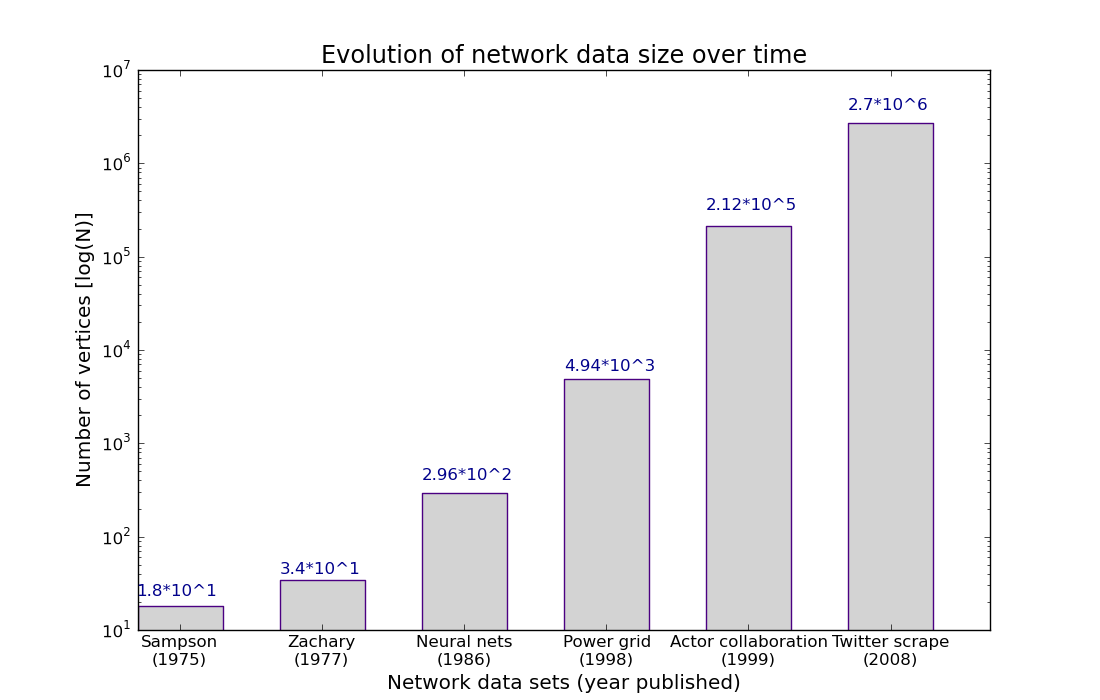
\includegraphics[scale=.37]{../images/figures/net_size_evo.png}
    \end{center}
    \uncover<2->{\alert{As network data becomes more readily available this trend will continue!}}
\end{frame}

\begin{frame}[fragile]
    \frametitle{How network size affects tools}
    While the data continues to scale up, many tools have not kept pace
    \vspace{2mm}
    \begin{center}
        \begin{tabular}{lcc}
            \multicolumn{3}{c}{\LARGE{Standard Tool Limitations}} \\ \hline\hline
            Tool & Node Limit & Platforms \\ \hline
            UCINet & \sim V=5K & Windows only\\
            Pajek & \sim V=100K & Windows only\\
            Statnet & \sim V= & Multi-platform \\
            ORA & \sim V=  & Window \& Linux
        \end{tabular}
        \uncover<2->{\begin{columns}
            \column{.5\textwidth}
            NetworkX is designed to handle data sets of the scale being generated today
            \begin{itemize}
                \item 10's of millions or nodes and 100's of millions of edges
                \item Can read network data from local files, or from external sources
                \begin{itemize}
                    \item Internet
                    \item Relational databases 
                \end{itemize}
                \item Inherently mutli-platform
            \end{itemize}
            \column{.5\textwidth}
            \begin{center}
                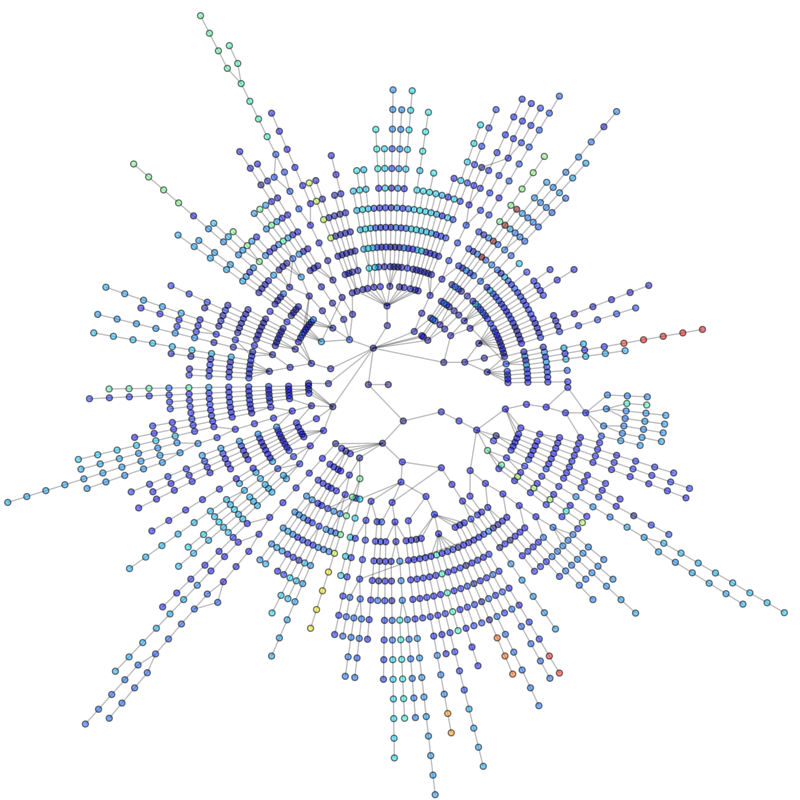
\includegraphics[scale=.21]{../images/networks/lanl_routes.png}
            \end{center}
        \end{columns}}
    \end{center}
\end{frame}

% subsection network_data_size_and_tool_scalabilty (end)

\subsection{Supporting non-traditional graph types} % (fold)
\label{sub:supporting_non_traditional_graph_types}

\begin{frame}[fragile]
    \frametitle{Moving beyond basic concepts of the ``graph''}
    In a more fundamental way, however, most network tools are limited in their concept of what can be a network
    \begin{itemize}
        \item Networks are collections of nodes and edges
        \item Nodes are static integers or strings, and edges are binary or continuous values
    \end{itemize}
    NetworkX can represent \textbf{ANY} relationship supported by Python data types
    \vspace{2mm}
    \begin{columns}
        \column{.3\textwidth}
        \small{Suppose we had data, or a data generating process, that was a time-series
        \begin{itemize}
            \item Current tools need kludges or hacks to add this data
            \item In NetworkX, we simply use the built-in Python \texttt{datetime} package to create a network of time-stamps
        \end{itemize}}
        \column{.7\textwidth}
        \begin{block}{\scriptsize{Simple time-series network}}
            \begin{code}
\tiny{G=DiGraph()
\alert<2>{# Create datetime object nodes}
for v in xrange(num_nodes):
    G.add_node(datetime.now())
time_nodes=G.nodes()
\alert<3>{# Add edges with `time' attribute}
for i in xrange(num_nodes):
    draws=random.uniform(0,1,num_nodes)
    for j in xrange(num_nodes):
        if i!=j and draws[j]<=p:
            G.add_edge(time_nodes[i],time_nodes[j],time=datetime.now())
...
\alert<4>{# target source datetime_created}
2010-05-25 13:38:42.515323 2010-05-25 13:38:42.515492 
    \{`time': datetime.datetime(2010, 5, 25, 13, 38, 42, 515752)\}
...}
                \end{code}
            \end{block}
    \end{columns}
\end{frame}

% subsection supporting_non_traditional_graph_types (end)

% section speed_and_scalability (end)

\section{Scientific computing in Python} % (fold)
\label{sec:scientific_computing_in_python}

\subsection{SciPy, NumPy and matplotlib} % (fold)
\label{sub:scipy_numpy_and_matplotlib}

\begin{frame}[fragile]
    \frametitle{Python's scientific computing holy trinity}
    \begin{columns}
        \column{.33\textwidth}
        \begin{center}
            \href{http://www.scipy.org}{
\includegraphics[width=3cm]{../images/logos/Scipylogo.png}}
        \end{center}
        \uncover<2->{Python's primary library for \textbf{mathematical and statistical} computing. Containing sub-libs for
        \begin{itemize}
            \item Numeric optimization
            \item Clustering
            \item Linear algebra
            \item ..and many others
        \end{itemize}}
        \uncover<3->{The primary data type in \texttt{SciPy} is an array
        \begin{itemize}
            \item Data manipulation is similar to that of MATLAB
        \end{itemize}}
        \vspace{3mm}
        \column{.33\textwidth}
        \begin{center}
            \href{http://numpy.scipy.org/}{
\includegraphics[clip,trim=0mm 2mm 0mm 2mm,width=2.5cm]{../images/logos/NumPy_logo.png}}
        \end{center}
        \uncover<4->{\texttt{NumPy} is an extension of the \texttt{SciPy} data type to include \textbf{multidimensional arrays and matrices}
        \begin{itemize}
            \item Provides many functions for working on arrays and matrices
            \item Very useful for representing relational data
        \end{itemize}}
        \uncover<5->{Both \textttt{SciPy} and \texttt{NumPy} rely on the C library \texttt{LAPACK} for very fast implementation}
        \column{.33\textwidth}
        \begin{center}
            \href{http://matplotlib.sourceforge.net/}{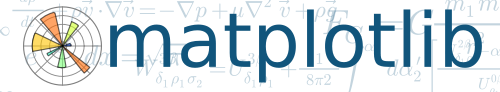
\includegraphics[width=3cm]{../images/logos/500px-Matplotlib_logo.png}}
        \end{center}
        \uncover<6->{\texttt{matplotlib} is \textbf{primary plotting library in Python}
        \begin{itemize}
            \item Supports 2- and 3-D plotting
            \item API allows embedding in apps
        \end{itemize}}
        \uncover<7->{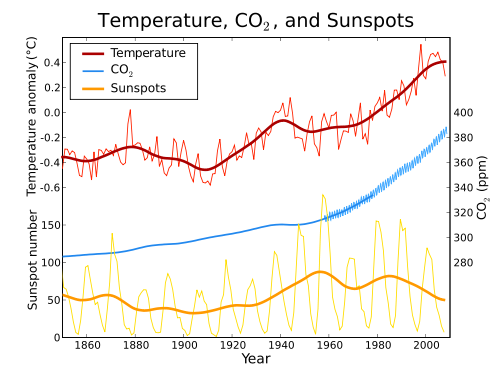
\includegraphics[width=2cm]{../images/figures/500px-Temp-sunspot-co2.png}
        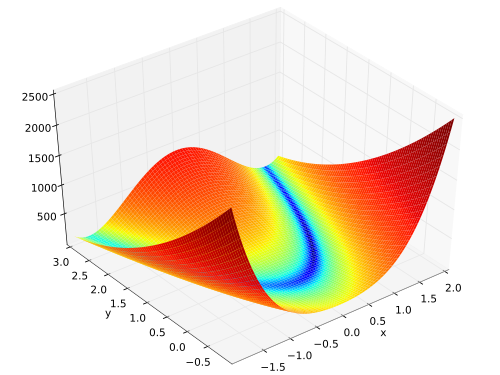
\includegraphics[width=2cm]{../images/figures/500px-Rosenbrock_function.png}}\\
        \uncover<8->{All graphics are highly customizable and professional publication ready}
    \end{columns}
    \vspace{1mm}
    \uncover<9->{\alert{NetworkX uses this entire suite to store, analyze and visualize networks}}
\end{frame}

% subsection scipy_numpy_and_matplotlib (end)

\subsection{Working with GraphViz} % (fold)
\label{sub:working_with_graphviz}

\begin{frame}[fragile]
    \frametitle{Exporting to GraphViz in NetworkX}
    NetworkX is designed to be an open-source all-purpose network manipulation and analysis tool
    \begin{itemize}
        \item Historically, the focus has not been on visualization
    \end{itemize}
    While there are several options for visualization in NetworkX, perhaps the best is its ability to read and write \texttt{GraphViz} files
    \begin{itemize}
        \item GraphViz is an open-source tool designed specifically for drawing graphs from the DOT language
        \item NetworkX works directly with GV using the \texttt{pygraphviz} package
    \end{itemize}
    \begin{columns}
        \column{.68\textwidth}
        \begin{block}{\scriptsize{Load Sampson data and visualize with graphviz}}
            \begin{code}
\tiny{\alert<2>{# Load Sampson monastery data from edglist}
>>> g2=read_edgelist("samp_like_el.txt",delimiter="\textbackslash t",create_using=DiGraph())
>>> info(g2)
Name:                  
Type:                  DiGraph
Number of nodes:       18
Number of edges:       55
Average in degree:     3.0556
Average out degree:    3.0556
\alert<3>{# Convert to pygraphviz type}
>>> g2_gv=to_agraph(g2)
\alert<4>{# Output DOT file and draw using dot layout}
>>> g2_gv.write("samp_like_dot.dot")
>>> g2_gv.draw('samp_like.png',prog='dot')}
            \end{code}
        \end{block}
        \column{.32\textwidth}
        \begin{center}
            \uncover<5->{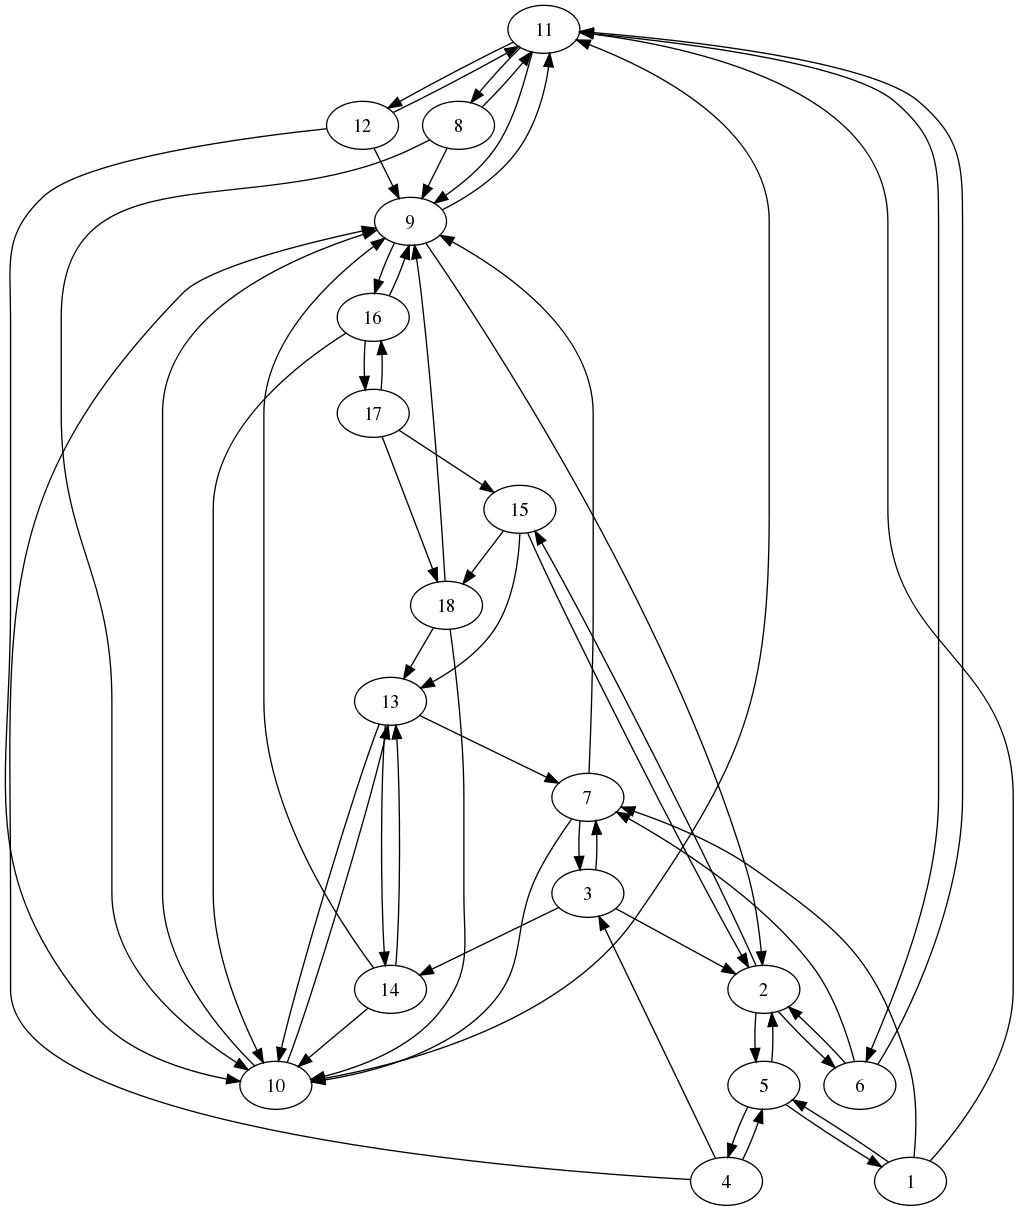
\includegraphics[height=4cm]{../images/networks/samp_like.png}}
        \end{center}
    \end{columns}
\end{frame}

% subsection working_with_graphviz (end)

% section scientific_computing_in_python (end)

\end{document}
